\documentclass[14pt,aspectratio=1610]{beamer}

\usepackage[brazil]{babel}
\usepackage[utf8]{inputenc}
%\UseRawInputEncoding
\usepackage[T1]{fontenc}
\usepackage{Sweave}
\usepackage{animate}
\usepackage{amsbsy}
\usepackage{amsfonts}
\usepackage{amsmath}
\usepackage{amssymb}
\usepackage{amsthm}
\usepackage[toc,page,title,titletoc]{appendix}
\usepackage[fixlanguage]{babelbib}
%\usepackage[pdftex]{color}
\usepackage{dsfont}
\usepackage{esvect}
\usepackage[labelfont=bf]{caption}
\usepackage{float}
\usepackage[Glenn]{fncychap}%Sonny %Conny %Lenny %Glenn %Renje %Bjarne %Bjornstrup
%\usepackage{geometry, calc, color, setspace}%
%\geometry{a4paper, headsep=1.0cm, footskip=1cm, lmargin=3cm, rmargin=2cm, tmargin=3cm, bmargin=2cm}
\usepackage{graphicx}
\usepackage{indentfirst}%Para indentar os parágrafos automáticamente
\usepackage{lipsum}
\usepackage{longtable}
\usepackage{mathtools}
\usepackage{listings}%Inserir codigo do R no latex
\usepackage{multirow}
\usepackage{multicol}
\usepackage{natbib}
\bibliographystyle{abbrvnat3}
\usepackage[figuresright]{rotating}
\usepackage{spalign}
%\usepackage{pgfpages}
\usepackage{pgfplots}
\usepackage{tikz}
\usepackage{color, colortbl}
\usepackage{ragged2e}%para justificar o texto dentro de algum ambiente
\definecolor{Gray}{gray}{0.9}
\definecolor{LightCyan}{rgb}{0.88,1,1}


\usepackage[all]{xy}
\usepackage{hyperref,bookmark}
\hypersetup{
  colorlinks=true,
  linkcolor=blue,
  citecolor=red,
  filecolor=blue,
  urlcolor=blue,
}

\usetheme{Boadilla}
%\usecolortheme[RGB={193,0,0}]{structure}

%\setbeamertemplate{footline}[frame number]
%\setbeamertemplate{footline}[text line]{%
%  \parbox{\linewidth}{\vspace*{-8pt}\hfill\date{}\hfill\insertshortauthor\hfill\insertpagenumber}}
\beamertemplatenavigationsymbolsempty
\renewcommand{\vec}[1]{\mbox{\boldmath$#1$}}
\newtheorem{Teorema}{Teorema}
\newtheorem{Proposicao}{Proposição}
\newtheorem{Definicao}{Definição}
\newtheorem{Corolario}{Corolário}
\newtheorem{Demonstracao}{Demonstração}
\newcommand{\bx}{\ensuremath{\bar{x}}}
\newcommand{\Ho}{\ensuremath{H_{0}}}
\newcommand{\Hi}{\ensuremath{H_{1}}}


\apptocmd{\frame}{}{\justifying}{} % Allow optional arguments after frame.

\title{MAF 261 - Estatística Experimental}
\author{Prof. Fernando de Souza Bastos}
\institute{Instituto de Ciências Exatas e Tecnológicas\texorpdfstring{\\ Universidade Federal de Viçosa}{}\texorpdfstring{\\ Campus UFV - Florestal}{}}
\date{2018}
\newcommand\mytext{Aula 8}
\newcommand\mytextt{Fernando de Souza Bastos}
\makeatletter
\setbeamertemplate{footline}
{
  \leavevmode%
  \hbox{%
  \begin{beamercolorbox}[wd=.333333\paperwidth,ht=2.25ex,dp=1ex,center]{author in head/foot}%
    \usebeamerfont{author in head/foot}\mytext
  \end{beamercolorbox}%
  \begin{beamercolorbox}[wd=.333333\paperwidth,ht=2.25ex,dp=1ex,center]{title in head/foot}%
    \usebeamerfont{title in head/foot}\mytextt
  \end{beamercolorbox}%
  \begin{beamercolorbox}[wd=.333333\paperwidth,ht=2.25ex,dp=1ex,right]{date in head/foot}%
    \usebeamerfont{date in head/foot}\insertshortdate{}\hspace*{2em}
    \insertframenumber{} / \inserttotalframenumber\hspace*{2ex} 
  \end{beamercolorbox}}%
  \vskip0pt%
}
\makeatother


\providecommand{\arcsin}{} \renewcommand{\arcsin}{\hspace{2pt}\textrm{arcsen}}
\providecommand{\sin}{} \renewcommand{\sin}{\hspace{2pt}\textrm{sen}}
%\newtheorem{Teorema}{Teorema}
%\newtheorem{Proposicao}{Proposição}
%\newtheorem{Definicao}{Definição}
%\newtheorem{Corolario}{Corolário}
%\newtheorem{Demonstracao}{Demonstração}

% Layout da pagina
\hypersetup{pdfpagelayout=SinglePage}
\begin{document}
\Sconcordance{concordance:Aula15.tex:Aula15.Rnw:%
1 238 1 1 18 1 3 28 1 1 18 1 3 461 1}


\frame{\titlepage}

\begin{frame}{}
\frametitle{\bf Sumário}
\tableofcontents
\end{frame}

\section{Experimentos Fatoriais}
\begin{frame}{Experimentos Fatoriais}
\frametitle{}
\begin{block}{}
\justifying
Experimentos fatoriais são aqueles em que se estudam simultaneamente
dois ou mais fatores, cada um deles com dois ou mais níveis.
\end{block}
\pause
\begin{block}{}
\justifying
O fatorial é um tipo de esquema, ou seja, uma das maneiras de organizar os tratamentos e não um tipo de delineamento, que representa a maneira pela qual os
tratamentos são distribuídos às unidades experimentais.
\end{block}
\pause
\begin{block}{}
\justifying
Na verdade, os experimentos fatoriais são montados segundo um tipo de delineamento
experimental, como por exemplo: o DIC e o DBC.
\end{block}
\end{frame}

\begin{frame}{}
\frametitle{}
\begin{block}{}
\justifying
Nos experimentos fatoriais, os tratamentos são obtidos pelas combinações
dos níveis dos fatores.
\end{block}
\pause
\begin{block}{}
\justifying
Num experimento fatorial completo, cada nível de um fator combina com todos os níveis dos outros fatores.
\end{block}
\pause
\begin{block}{}
\justifying
A principal aplicação de experimentos fatoriais é quando se quer saber sobre o efeito de diversos fatores que influenciam na variável em estudo e o relacionamento entre eles.
\end{block}
\end{frame}

\begin{frame}{}
\frametitle{}
\begin{block}{}
\justifying
A simbologia comumente utilizada, para experimentos fatoriais é indicar
o produto dos níveis dos fatores em teste. Por exemplo: Experimento Fatorial
$2x4x6.$ O produto $2x4x6$ informa que no experimento foram testados
simultaneamente 3 fatores. O primeiro possui 2 níveis, o segundo 4 níveis e o
terceiro 6 níveis.
\end{block}
\pause
\begin{block}{}
\justifying
Quando o número de níveis é igual para todos os fatores, pode-se utilizar a seguinte simbologia: $n^{F},$ em que $F$ é o número de fatores $n$ é o número de níveis de cada fator. Por exemplo: Experimento Fatorial $4^{3}.$ A potência $4^{3}$ informa que o experimento tem 3 fatores com 4 níveis cada um.
\end{block}
\end{frame}

\section{Efeitos avaliados em um experimento fatorial}
\begin{frame}{Tipos de efeitos avaliados em um experimento fatorial}
\frametitle{}
\begin{block}{}
\justifying
Nos experimentos fatoriais, podem ser estudados os seguintes efeitos:
\begin{itemize}
\item {\bf Efeito Principal:} é o efeito de cada fator, independente do efeito dos
outros fatores;\pause
\item {\bf Efeito de Interação:} é o efeito simultâneo dos fatores sobre a variável
em estudo. Dizemos que ocorre interação entre os fatores quando os efeitos
dos níveis de um fator são modificados pelos níveis do outro fator.
\end{itemize}
\end{block}
\end{frame}

\begin{frame}{}
\frametitle{}
\begin{block}{}
\justifying
O efeito da interação pode ser mais facilmente compreendido por meio
de gráficos. Para ilustrar o efeito da interação, considere um experimento
fatorial $3x2,$ em que os fatores em testes são Variedade (V) e Espaçamento
(E). Os tratamentos para este experimento são os seguintes:
\begin{table}[!h]
\begin{tabular}{ccc}
V1E1&V2E1&V3E1\\
V1E2&V2E2&V3E2
\end{tabular}
\end{table}
\end{block}
\end{frame}

\begin{frame}{}
\frametitle{}
\begin{block}{}
\justifying
Suponha os seguintes resultados fictícios, para a variável altura de
plantas (cm), deste experimento, nas seguintes situações:
\begin{table}[!h]
\begin{tabular}{cccc}
\hline
&\multicolumn{3}{c}{Variedades}\\
\cline{2-4}
Espaçamentos&$V1$&$V2$&$V3$\\
\hline
$E1$&8&10&12\\
$E2$&6&8 &10\\
\hline
\end{tabular}
\end{table}
Quando não há interação as diferenças entre os resultados dos níveis de
um fator são estatisticamente iguais para todos os níveis do outro fator.
\end{block}
\end{frame}

\begin{frame}{}
\frametitle{}
\begin{block}{}
\begin{center}
\setkeys{Gin}{width=0.5\linewidth}
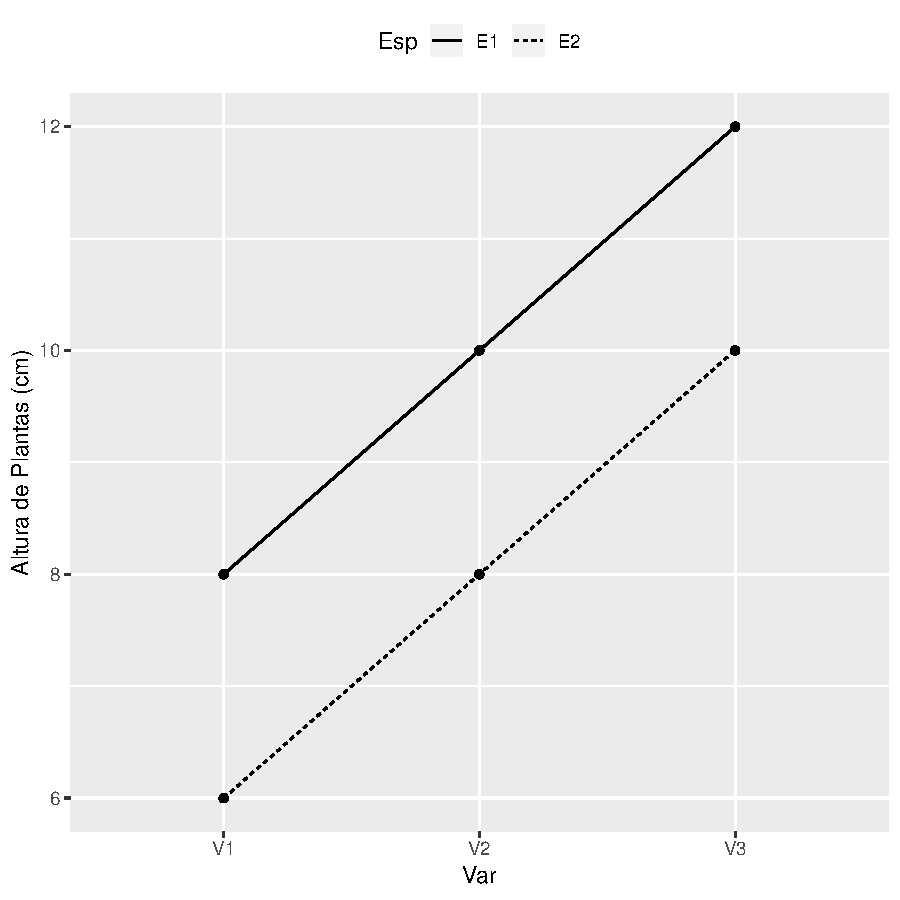
\includegraphics{Aula15-001}
\end{center}
\end{block}
\end{frame}

\begin{frame}{}
\frametitle{}
\begin{block}{}
\justifying
\begin{table}[!h]
\begin{tabular}{cccc}
\hline
&\multicolumn{3}{c}{Variedades}\\
\cline{2-4}
Espaçamentos&$V1$&$V2$&$V3$\\
\hline
$E1$&2&4&6\\
$E2$&5&10&2\\
\hline
\end{tabular}
\end{table}
Quando há interação as diferenças entre os níveis de um fator dependem dos níveis do outro fator.
\end{block}
\end{frame}

\begin{frame}{}
\frametitle{}
\begin{block}{}
\begin{center}
\setkeys{Gin}{width=0.5\linewidth}
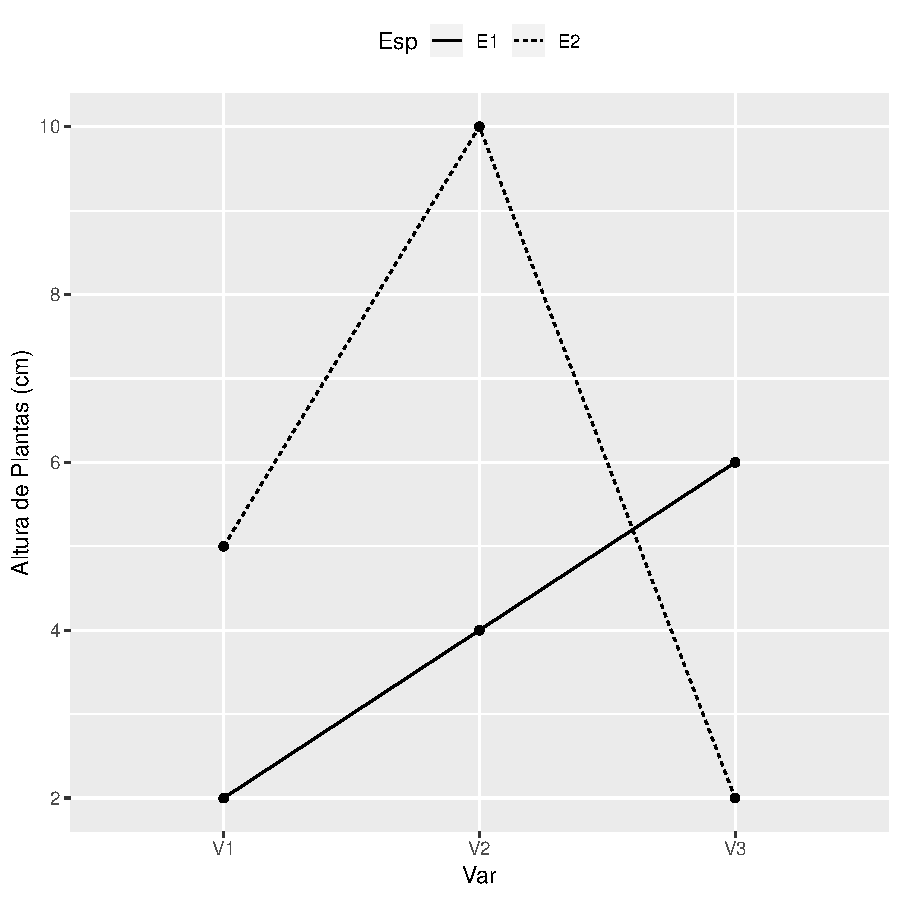
\includegraphics{Aula15-002}
\end{center}
\end{block}
\end{frame}

\section{Tabulação dos dados}
\begin{frame}{}
\frametitle{}
\begin{block}{}
\justifying
Uma maneira de tabular os dados de um experimento fatorial, com dois fatores
$A$ e $B,$ com $I$ e $J$ níveis, respectivamente, instalados segundo o DIC, com $K$
repetições, é fornecida a seguir:
\begin{figure}[H]
    \centering
    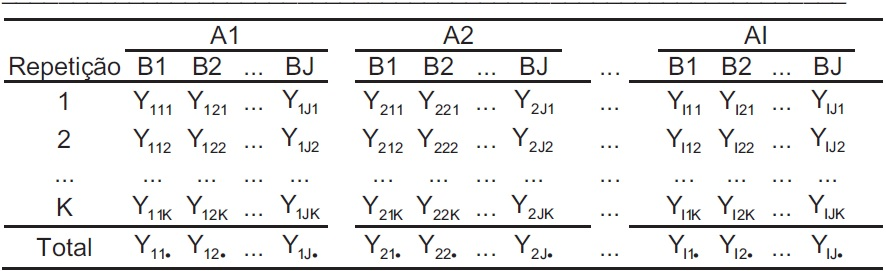
\includegraphics[scale=0.5]{Figuras/Tabulacao}
    %\caption{}
    %\label{figRotulo}
  \end{figure}
\end{block}
\end{frame}

\begin{frame}{}
\frametitle{}
\begin{block}{}
\justifying
Pode-se montar um quadro auxiliar contendo os totais de tratamentos,
cujos valores são obtidos pela soma de todas as repetições para o tratamento
em questão. Este quadro facilita o cálculo das somas de quadrados devido aos
fatores A e B, e da interação entre eles. Para a situação citada, o quadro de
totais de tratamentos é do seguinte tipo:
\begin{figure}[H]
    \centering
    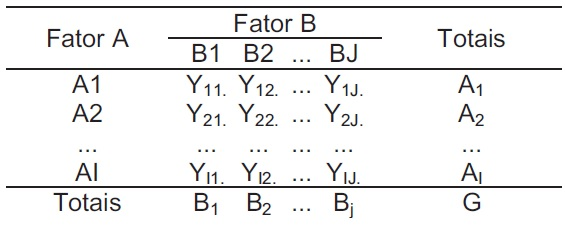
\includegraphics[scale=0.5]{Figuras/Tabulacao2}
    %\caption{}
    %\label{figRotulo}
  \end{figure}
\end{block}
\end{frame}

\section{Modelo Estatístico}
\begin{frame}{}
\frametitle{}
\begin{block}{}
\justifying
Considere um experimento fatorial, com dois fatores: o fator A com $I$
níveis e o fator B com $J$ níveis, instalados segundo o DIC, com $K$ repetições. O
modelo estatístico para um experimento como este é:
$$Y_{ijk}=\mu+\alpha_{i}+\beta_{j}+(\alpha\beta)_{ij}+e_{ijk}$$
em que, $Y_{ijk}$ é o valor observado para a variável em estudo referente a k-ésima
repetição da combinação do i-ésimo nível do fator A com o j-ésimo
nível do fator B; $\alpha_{i}$ é o efeito do i-ésimo nível do fator A no valor observado $Y_{ijk}$; $\beta_{j}$ é o efeito do j-ésimo nível do fator B no valor observado $Y_{ijk}$; $(\alpha\beta)_{ij}$ é o efeito da interação do i-ésimo nível do fator A com o j-ésimo nível do fator B;
\end{block}
\end{frame}

\begin{frame}{}
\frametitle{}
\begin{block}{}
\justifying
Para um experimento fatorial instalado segundo o DBC, com K blocos, o
modelo estatístico seria:
$$Y_{ijk}=\mu+\alpha_{i}+\beta_{j}+(\alpha\beta)_{ij}+\omega_{k}+e_{ijk}$$
em que, $\omega_{k}$ é o efeito do k-ésimo bloco na observação $Y_{ijk}.$
\end{block}
\end{frame}

\section{Análise de Variância}
\begin{frame}{}
\frametitle{}
\begin{block}{}
\justifying
A análise de variância de um experimento fatorial é feita desdobrando-se a
soma de quadrados de tratamentos nas partes devido aos efeitos principais de
cada fator e na parte devido à interação entre os fatores.
\end{block}
% \pause
% \begin{block}{}
% \justifying
% O quadro a seguir apresenta como seria a análise de um experimento
% fatorial, com 2 fatores A e B, com I e J níveis, respectivamente, e K repetições,
% instalado segundo o DIC.
% \end{block}
\end{frame}

\begin{frame}{}
\frametitle{}
\begin{block}{}
\justifying
O quadro a seguir apresenta como seria a análise de um experimento
fatorial, com 2 fatores A e B, com I e J níveis, respectivamente, e K repetições,
instalado segundo o DIC.
\end{block}
\pause
\begin{block}{}
\begin{table}[!h]
\scalebox{0.7}{%
\setlength{\arrayrulewidth}{2pt}
\begin{tabular}{cccccc}
\hline
FV&GL&SQ&QM&F&$F_{tab;\alpha}$\\
\hline
&&&&&\\
 A         &$(I-1)$     &SQA  & $-$ & $-$ & $-$\\
&&&&&\\
 B         &$(J-1)$     &SQB  & $-$ & $-$ & $-$\\
 &&&&&\\
$A\times B$&$(I-1)(J-1)$&SQInt& $\dfrac{SQInt}{(I-1)(J-1)}$ & $\dfrac{QMInt}{QMRes}$ & $[(I-1)(J-1);n_{2}]$\\
&&&&&\\
\hline
(Trat)&$(IJ-1)$&(SQTrat)&$-$&$-$&$-$\\
&&&&&\\
Resíduo&$n_{2}=IJ(K-1)$&SQRes&$\dfrac{SQRes}{IJ(K-1)}$&$-$&$-$\\
\hline
Total&$IJK-1$&SQTotal&$-$&$-$&$-$\\
\hline
\end{tabular}
}
\end{table}
\end{block}
\end{frame}

\begin{frame}{}
\frametitle{}
\begin{block}{}
\justifying
As fórmulas para a obtenção das somas de quadrados são as seguintes:

\begin{align*}
SQTotal&={\displaystyle \sum_{i=1,j=1,k=1}^{I,J,K}Y_{ijk}^{2}-C} &\quad& 
C=\dfrac{\Biggl({\displaystyle \sum_{i=1,j=1,k=1}^{I,J,K}Y_{ijk}\Biggl)^{2}}}{IJK}\\
SQTrat&={\displaystyle \sum_{i=1,j=1}^{I,J}\dfrac{Y_{ij.}^{2}}{k}-C} &\quad& 
SQA={\displaystyle \sum_{i=1}^{I}\dfrac{A_{i}^{2}}{JK}-C}\\
SQB&={\displaystyle \sum_{j=1}^{J}\dfrac{B_{j}^{2}}{IK}-C} &\quad& 
SQInt=SQTrat-SQA-SQB\\
SQResiduo&=SQTotal-SQTrat &\quad& 
 \\
\end{align*}

\end{block}
\end{frame}

\begin{frame}{}
\frametitle{}
\begin{block}{}
\justifying
O quadro abaixo apresenta como seria a análise de um experimento
fatorial, com 2 fatores A e B, com I e J níveis, respectivamente, e K repetições
(ou blocos), instalado segundo o DBC.
\end{block}
\pause
\begin{block}{}
\begin{table}[!h]
\scalebox{0.7}{%
\setlength{\arrayrulewidth}{2pt}
\begin{tabular}{cccccc}
\hline
FV&GL&SQ&QM&F&$F_{tab;\alpha}$\\
\hline
&&&&&\\
 A         &$(I-1)$     &SQA  & $-$ & $-$ & $-$\\
&&&&&\\
 B         &$(J-1)$     &SQB  & $-$ & $-$ & $-$\\
 &&&&&\\
$A\times B$&$(I-1)(J-1)$&SQInt& $\dfrac{SQInt}{(I-1)(J-1)}$ & $\dfrac{QMInt}{QMRes}$ & $[(I-1)(J-1);n_{2}]$\\
&&&&&\\
\hline
(Trat)&$(IJ-1)$&(SQTrat)&$-$&$-$&$-$\\
&&&&&\\
Blocos&$k-1$&SQBlocos&$-$&$-$&$-$\\
&&&&&\\
Resíduo&$n_{2}=(IJ-1)(K-1)$&SQRes&$\dfrac{SQRes}{(IJ-1)(K-1)}$&$-$&$-$\\
\hline
Total&$IJK-1$&SQTotal&$-$&$-$&$-$\\
\hline
\end{tabular}
}
\end{table}
\end{block}
\end{frame}

\begin{frame}{}
\frametitle{}
\begin{block}{}
\justifying
Nesta situação,

$$SQBlocos={\displaystyle \sum_{k=1}^{K}\dfrac{\omega_{k}^{2}}{IJ}-C}$$
em que, $\omega_{k}={\displaystyle \sum_{i=1,j=1}^{I,J}Y_{ijk}=Y_{..k}}$

\end{block}
\end{frame}

\begin{frame}{}
\frametitle{}
\begin{block}{}
\justifying
Conforme apresentado nas duas tabelas anteriores, na análise dos dados
oriundos de um experimento fatorial, para os dois tipos de delineamentos,
deve-se inicialmente proceder ao teste F para a interação entre os fatores. As
hipóteses para o teste F da interação são:
\end{block}
\pause
\begin{block}{}
\justifying
$H_{0}:$ Os fatores A e B atuam independentemente sobre a variável
resposta em estudo.

$H_{1}:$ Os fatores A e B não atuam independentemente sobre a variável
resposta em estudo.

\end{block}
\end{frame}

\begin{frame}{}
\frametitle{}
\begin{block}{}
\justifying
O resultado deste teste F para a interação indica como as comparações dos
níveis de um fator devem ser realizadas. Temos dois resultados possíveis para
o teste F da interação os quais serão apresentados a seguir.

\end{block}
\end{frame}

\section{Interação não-significativa}
\begin{frame}{Interação não-significativa}
\frametitle{}
\begin{block}{}
\justifying
Este caso ocorre quando a hipótese $H_{0}$ para a interação entre os fatores
não é rejeitada. Este resultado implica que os efeitos dos fatores atuam de
forma independente.
\end{block}
\pause
\begin{block}{}
\justifying
Portanto recomenda-se que as comparações dos níveis de um fator
sejam feitas de forma geral em relação ao outro fator, ou seja, independente
dos níveis outro fator. O passo seguinte na análise estatística dos dados
experimentais é proceder ao teste F para cada fator como ilustrado na tabela
apresentada a seguir para o caso do DBC.
\end{block}
\end{frame}

\begin{frame}{}
\frametitle{}
\begin{block}{}
\begin{table}[!h]
\scalebox{0.7}{%
\setlength{\arrayrulewidth}{2pt}
\begin{tabular}{cccccc}
\hline
FV&GL&SQ&QM&F&$F_{tab;\alpha}$\\
\hline
&&&&&\\
 A         &$(I-1)$     &SQA  & $\dfrac{SQA}{(I-1)}$ & $\dfrac{QMA}{QMRes}$ & $[(I-1),n_{2}]$\\
&&&&&\\
 B         &$(J-1)$     &SQB  & $\dfrac{SQB}{(J-1)}$ & $\dfrac{QMB}{QMRes}$ & $[(J-1),n_{2}]$\\
 &&&&&\\
$A\times B$&$(I-1)(J-1)$&SQInt& $\dfrac{SQInt}{(I-1)(J-1)}$ & Não- & $-$\\
&&&&Significativo&\\
\hline
(Trat)&$(IJ-1)$&(SQTrat)&$-$&$-$&$-$\\
&&&&&\\
Blocos&$k-1$&SQBlocos&$-$&$-$&$-$\\
&&&&&\\
Resíduo&$n_{2}=(IJ-1)(K-1)$&SQRes&$\dfrac{SQRes}{(IJ-1)(K-1)}$&$-$&$-$\\
\hline
Total&$IJK-1$&SQTotal&$-$&$-$&$-$\\
\hline
\end{tabular}
}
\end{table}
\end{block}
\end{frame}

\begin{frame}{}
\frametitle{}
As hipóteses para realizar o teste F para os efeitos principais são:
\begin{block}{Fator A}
\justifying
$H_{0}:\mu_{A_{1}}=\cdots=\mu_{A_{I}},$ ou seja, todos os possíveis contrastes entre as médias dos níveis do fator A, são estatisticamente nulos, ao nível de probabilidade em que foi executado o teste.\\
$H_{1}:$ Não $H_{0}.$ Ou seja, existe pelo menos um contraste entre as médias dos
níveis do fator A, que é estatisticamente diferente de zero, ao nível de
probabilidade em que foi executado o teste.
\end{block}
\pause
\begin{block}{Fator B}
\justifying
$H_{0}:\mu_{B_{1}}=\cdots=\mu_{B_{J}}.$\\
$H_{1}:$ Não $H_{0}.$ Ou seja, existe pelo menos um contraste entre as médias dos
níveis do fator B, que é estatisticamente diferente de zero, ao nível de
probabilidade em que foi executado o teste.
\end{block}
\end{frame}

\begin{frame}{}
\frametitle{}
\begin{block}{}
\justifying
Se os fatores A e B forem qualitativos, e o teste F para A e/ou B, for não
significativo, a aplicação do teste de médias é desnecessária. Se o teste F for
significativo, para A e/ou B, aplica-se um teste de médias para comparar os
níveis do fator. As estimativas das médias dos níveis dos fatores são obtidas
por:

$$\hat{\mu}_{A_{i}}=\dfrac{A_{i}}{JK}\quad \hat{\mu}_{B_{j}}=\dfrac{B_{j}}{IK}$$

\end{block}
\end{frame}

\section{Interação significativa}
\begin{frame}{Interação significativa}
\frametitle{}
\begin{block}{}
\justifying
Este caso ocorre quando a hipótese $H_{0}$ para a interação entre os fatores
é rejeitada. Este resultado implica que os efeitos dos fatores atuam de forma
dependente. Neste caso as comparações entre os níveis de um fator levam em
consideração o nível do outro fator, pois o resultado significativo para a
interação indica que o efeito de um fator depende do nível do outro fator.
\end{block}
\end{frame}

\begin{frame}{}
\frametitle{}
\begin{block}{}
\justifying
Portanto, não é recomendado realizar o teste F para cada fator
isoladamente tal como foi apresentado para o caso da interação não significativa.
O procedimento recomendado é realizar o desdobramento do
efeito da interação.
\end{block}
\end{frame}

\begin{frame}{}
\frametitle{}
\begin{block}{}
\justifying
Para realizar este desdobramento deve-se fazer uma nova análise de
va\-ri\-ân\-cia em que os níveis de um fator são comparados dentro de cada nível
do outro fator, tal como apresentado nas tabelas a seguir.
\end{block}
\end{frame}

\begin{frame}{}
\frametitle{}
\begin{block}{}
\justifying
Desdobramento para comparar os níveis de A dentro de cada nível de B,
ou seja, estudar $A/B:$
\begin{figure}[H]
    \centering
    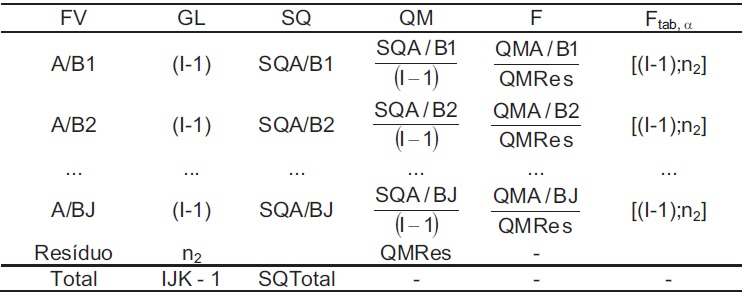
\includegraphics[scale=0.5]{Figuras/A_dentro_B}
    %\caption{}
    %\label{figRotulo}
  \end{figure}
\end{block}
\end{frame}

\begin{frame}{}
\frametitle{}
\begin{block}{}
\justifying
As hipóteses para testar as fontes de variação da tabela acima, para 
$j=1,2,3,\cdots,J,$ são:\\

$H_{0}:\mu_{A_{1}/B_{j}}=\mu_{A_{2}/B_{j}}=\cdots=\mu_{A_{I}/B_{j}}$\\
$H_{1}:$ Não $H_{0}$

\end{block}
\end{frame}

\begin{frame}{}
\frametitle{}
\begin{block}{}
\justifying
Desdobramento para comparar os níveis de B dentro de cada nível de A,
ou seja estudar $B/A$
\begin{figure}[H]
    \centering
    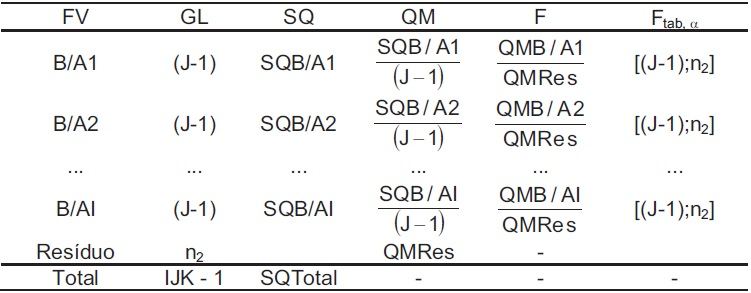
\includegraphics[scale=0.5]{Figuras/B_dentro_A}
    %\caption{}
    %\label{figRotulo}
  \end{figure}
\end{block}
\end{frame}

\begin{frame}{}
\frametitle{}
\begin{block}{}
\justifying
As hipóteses para testar as fontes de variação da tabela acima, para 
$i=1,2,3,\cdots,I,$ são:\\

$H_{0}:\mu_{B_{1}/B_{i}}=\mu_{B_{2}/A_{i}}=\cdots=\mu_{B_{J}/A_{i}}$\\
$H_{1}:$ Não $H_{0}$

\end{block}
\end{frame}

\begin{frame}{}
\frametitle{}
\begin{block}{}
\justifying
Se os fatores forem qualitativos, procede-se ao teste F para cada fonte de
variação do desdobramento. Nas fontes de variação em que o teste F foi
significativo e o fator tem mais de dois níveis, recomenda-se a aplicação de um
teste de médias. As estimativas das médias dos níveis dos fatores são obtidas
por
$$\hat{\mu}_{A_{i}}=\dfrac{A_{i}}{K}\quad \hat{\mu}_{B_{j}}=\dfrac{B_{j}}{K}$$
\end{block}
\end{frame}

\section{Conclusões}
\begin{frame}{Vantagens e desvantagem de um experimento fatorial}
\frametitle{}
\begin{block}{Vantagens}
\justifying
\begin{itemize}
\item Permite o estudo dos efeitos principais e o efeito da interação entre os
fatores.\pause
\item  O número de graus de liberdade associado ao resíduo é alto quando
comparado com os experimentos simples dos mesmos fatores, o que contribui para diminuir a variância residual, aumentando a precisão do experimento.
\end{itemize}
\end{block}
\pause
\begin{block}{Desvantagem}
\justifying
\begin{itemize}
\item Requer maior número de unidades experimentais em relação aos
experimentos simples.
\end{itemize}
\end{block}
\end{frame}

\section{Exemplo}
\begin{frame}{}
\frametitle{}
\begin{block}{Exemplo 8.1}
\justifying
Seja um experimento fatorial instalado no DIC, com dois fatores: Irrigação
(A) e Calagem (B), cada um deles com dois níveis: presença $(A_{1},B_{1})$ e
ausência $(A_{0},B_{0})$. Os dados obtidos (kg de planta/parcela) para cada
tratamento são fornecidos abaixo. Pede-se realizar a ANOVA e obter as
conclusões sobre os fatores. Use $\alpha=5\%.$
\end{block}

\begin{table}[!h]
\begin{tabular}{cccc}
\hline
$A_{0}B_{0}$&$A_{0}B_{1}$&$A_{1}B_{0}$&$A_{1}B_{1}$\\
\hline
25&35&41&60\\
32&28&35&67\\
27&33&38&59\\
\hline
\end{tabular}
\end{table}
\end{frame}


\end{document}
